\documentclass[border=3pt]{standalone}




\usepackage[usenames,dvipsnames]{xcolor}
\usepackage{fullpage}
\usepackage[upright]{fourier}
\usepackage{tkz-graph}
\usetikzlibrary{arrows}

\usepackage{newtxsf}
\usepackage[T1]{fontenc}
\usepackage[sfdefault]{FiraSans}
\begin{document}
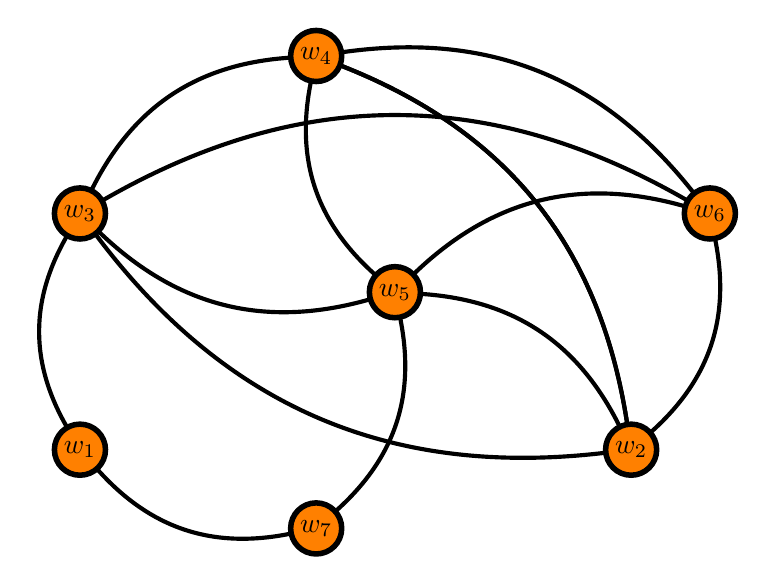
\begin{tikzpicture}
  \SetVertexNormal[Shape      = circle,
                   FillColor  = orange,
                   LineWidth  = 2pt]
  \SetUpEdge[lw         = 1.5pt,
             color      = black,
             labelcolor = white,
             labeltext  = red,
             labelstyle = {sloped,draw,text=blue}]
 \tikzstyle{EdgeStyle}=[bend left]
 \Vertex[x=0, y=0,L=$w_1$]{G}
 \Vertex[x=0, y=3,L=$w_3$]{A} 
 \Vertex[x=3, y=5,L=$w_4$]{P}
 \Vertex[x=4, y=2,L=$w_5$]{C}
 \Vertex[x=8, y=3,L=$w_6$]{Q}
 \Vertex[x=7, y=0,L=$w_2$]{E}
 \Vertex[x=3, y=-1,L=$w_7$]{R}
 \Edges(G,A,P,Q,E) \Edges(C,A,Q) \Edges(C,R,G) \Edges(P,E,A)
 \Edges(C,P,E) \Edges(C,E) \Edges(C,Q)
\end{tikzpicture}
\end{document}